
\section{Hamiltonian of a Transmon Network}\label{section:transmon_network_hamiltonian}
Here, we will consider an arbitrary $N$-port impedance of form (\ref{eq:impedance}) that is shunted by Josephson junctions as shown in Fig.\ \ref{fig:transmon_network}. At this point, we assume that any external ports are left open, but later on we will include them to estimate the Purcell decay rates of the qubits. We also assume that the impedance represents all of the transmon network except for the Josephson junctions, which we have added in afterwards. For example, the transmon shunt capacitances will be the shunt capacitances of the ports of the multiport impedance.

\begin{figure}[h!]
    \centering
    \begin{circuitikz}[line width=1pt]
        \ctikzset{bipoles/thickness=1, bipoles/length=1cm}
        \ctikzset { label/align = straight }
        
        % ----------------------------- Impedance Network ---------------------------- %
        \draw[rounded corners=.5cm] (0,2) -- (0,4.5) -- (5,4.5) -- (5,0) -- (0,0) -- (0,2);
        \node at (2.5,2.25) {$\vb{Z}(s) = \dfrac{\vb{R}_0}{s} + \displaystyle\sum_{k=1}^M \dfrac{s \vb{R}_k}{s^2 + \omega_{R_k}^2}$};

        % ------------------------------ Left Lower Port ----------------------------- %
        \draw (0,0.5) to[short, -o] (-0.5,0.5) -- (-1, 0.5) to[barrier=$E_{J_N}$] (-1,1.5) to[short, -o] (-0.5,1.5) -- (0,1.5);

        % ------------------------------ Left Upper Port ----------------------------- %
        \draw (0,3) to[short, -o] (-0.5,3) -- (-1, 3) to[barrier=$E_{J_1}$] (-1,4) to[short, -o] (-0.5,4) -- (0,4);

        \node at (-0.5,2.35) {$\vdots$};

    \end{circuitikz}
    \caption{Network of $N$ transmons represented by an arbitrary impedance function (\ref{eq:impedance}). The arbitrary impedance suggests that the transmons are coupled capacitively to each other and to resonant modes.}
    \label{fig:transmon_network}
\end{figure}

We can immediately write the circuit Hamiltoninan for Fig.\ \ref{fig:transmon_network} using the results of Section \ref{section:impedance_hamiltonian}. Now since we include the junctions, we use (\ref{eq:impedance_hamiltonian}) to find:
\begin{equation}\label{eq:transmon_hamiltonian}
    \mathcal{H} = \frac{1}{2} \vb{Q}^T \vb{C}^{-1} \vb{Q} + \frac{1}{2} \vb{\Phi}^T \vb{M} \vb{\Phi} - \sum_{i=1}^N E_{J_i} \cos(\frac{2\pi}{\Phi_0} \Phi_{J_i})
\end{equation}
Here we will represent the junction port fluxes using $\Phi_{J_i}$ instead of $\Phi_{P_i}$. Since the impedance function can also be represented as a CL cascade, we note that any analysis of Hamiltonian (\ref{eq:transmon_hamiltonian}) will also apply to transmon network built from arbitrary CL cascade. We can also promote our conjugate variables $\Phi_{i}$ and $Q_i$ to operators, such that they satisfy the commutation relation $[\hat{\Phi}_i, \hat{Q}_j] = i\hbar \delta_{ij}$. We next want to expand the Hamiltonian to obtain coupling rates between the different branches. Before doing this, we can introduce some notation that will help simplify our expressions. First, we define the effective port capacitance:
\begin{equation}\label{eq:effective_capacitiance}
    \tilde{C}_i = \frac{1}{(\vb{C}^{-1})_{ii}}
\end{equation}
With this we also define an effective charging energy $\tilde{E}_{C_i} = e^2/2\tilde{C}_i$. Generally, this charging energy is defined using just the branch shunt capacitance. However, since we have the full capacitance matrix, we can avoid this approximation. Note that from (\ref{eq:impedance_cap_inverse}) we can see that for the inductive branches, $\tilde{C}_{R_k} = 1$. We can also define an inductive energy for the inductive branches:
\begin{equation}
    E_{L_{k}} = \frac{\Phi_0^2}{4\pi^2 L_{R_k}}
\end{equation}
Next, we rescale the flux and charge variables: $\hat{\phi} = 2\pi\hat{\Phi}/\Phi_0$ and $\hat{q} = \hat{Q}/2e$. Their commutation relation is $[\hat{\phi}_i, \hat{q}_j] = i\delta_{ij}$. The Hamiltonian can now be rewritten using the above definitions:
\begin{align}
\begin{split}
    \hat{H} &= \sum_{i=1}^N \left(  4\tilde{E}_{C_i}\hat{q}_{J_i}^2 - E_{J_i}\cos(\hat{\phi}_{J_i})  + \sum_{j > i}^{j=N} 4e^2(\vb{C}^{-1})_{ij}\;  \hat{q}_{J_i}\hat{q}_{J_j} \right) \\
    &\quad + \sum_{k=1}^M \left( 4\tilde{E}_{C_i}\hat{q}_{R_k}^2 - \frac{E_{L_k}}{2}\hat{\phi}_{R_k}^2  + \sum_{\ell > k}^{\ell = M} 4e^2(\vb{C}^{-1})_{k\ell}\;  \hat{q}_{R_k}\hat{q}_{R_\ell} \right) \\ 
    &\quad + \sum_{i=1}^N \sum_{k=1}^M 4e^2(\vb{C}^{-1})_{ik}\; \hat{q}_{J_i}\hat{q}_{R_k}
\end{split}
\end{align}
Note that above and in the following, we will use the index labels $i$ and $j$ to refer to the transmon or junction branches. We will use the labels $k$ and $\ell$ to refer to the internal resonant or inductive branches. Next, we introduce creation and annihilation operators that will correspond to the transmons ($\opbd$ and $\hat{b}$) or resonator ($\opad$ and $\hat{a}$) branches. Since the operators are bosonic, they have the commutation relations $[\opb_i, \opbd_j]=\delta_{ij}$ and $[\opa_k, \opad_\ell]=\delta_{k\ell}$. We can rewrite our operators $\hat{\phi}_{J_i}$ and $\hat{q}_{J_i}$ in terms of the annihilation and creation operators $\opbd$ and $\hat{b}$:
\begin{align}
    \hat{\phi}_{J_i} &= \Bigg( \frac{2\tilde{E}_{C_i}}{E_{J_i}} \Bigg)^{\!\!1/4} (\opbd_{i} + \opb_{i}) \\
    \hat{q}_{J_i} &= \Bigg( \frac{2E_{J_i}}{\tilde{E}_{C_i}} \Bigg)^{\!\!1/4} (\opbd_{i} - \opb_{i})
\end{align}
The operators $\hat{\phi}_{R_k}$ and $\hat{q}_{R_k}$ can be rewritten in a similar way with $E_{L_k}$ instead of $E_J$. We can again rewrite the Hamiltonian in terms of these new bosonic operators:
\begin{align}
\begin{split}\label{eq:transmon_resonator_ham}
    \frac{1}{\hbar}\hat{H} &= \sum_{i=1}^N \left(  \omega_{J_i}\opbd_i\opb + \frac{\beta_{J_i}}{2}\opbd_i\opbd_i\opb_i\opb_i  + \sum_{j > i}^{j=N} g_{ij} (\opbd_i\opb_j + \opb_i\opbd_j - \opbd_i\opbd_j - \opb_i\opb_j) \right) \\
    &\quad + \sum_{k=1}^M \left( \omega_{R_k}\opad_k\opa_k + \sum_{\ell > k}^{\ell=M} g_{R_k,R_\ell} (\opad_k\opa_\ell + \opa_k\opad_\ell - \opad_k\opad_\ell - \opa_k\opa_\ell) \right) \\ 
    &\quad + \sum_{i=1}^N \sum_{k=1}^M g_{i,R_k}(\opbd_i\opa_k + \opb_i\opad_k - \opbd_i\opad_k - \opb_i\opa_k)
\end{split}
\end{align}

Above we have neglected constant terms and used the Duffing oscillator approximation to represent the transmon as a harmonic oscillator with a quartic perturbation \cite{transmon}. In the above Hamiltonian, we also have the following quantities:
\begin{alignat}{2}
    &\hbar\;\omega_{J_i} &&= \sqrt{8E_{J_i}\tilde{E}_{C_i}} + \beta_{J_i} \\
    &\hbar\;\beta_{J_i} &&= -\tilde{E}_{C_i} \\
    &\hbar\;\omega_{R_k} &&= \sqrt{8E_{L_k}\tilde{E}_{C_k}} \\
    &\hbar\; g_{ij} &&= e^2 (\vb{C}^{-1})_{ij} \left( \frac{E_{J_i} E_{J_j}}{4 \tilde{E}_{C_i} \tilde{E}_{C_j}  } \right)^{\!\!1/4} \label{eq:node_coupling}
\end{alignat}
The other coupling rates $g_{R_k,R_\ell}$ and $g_{i,R_k}$ are defined similarly but $E_J$ is replaced with $E_L$ as needed. For the impedance case, all couplings between the internal resonant modes will be zero since the resonator block in (\ref{eq:impedance_cap_inverse}) is the identity. Here, we leave the coupling term since this allows us to treat the general CL cascade case. This form of the Hamiltonian immediately gives us the coupling rates between all the qubits and resonant modes in the circuit. Thus, if we start with a CL cascade network or a rational impedance function (\ref{eq:impedance}), we can immediately compute the qubit frequencies as well as the coupling rates between the qubits and the other resonant modes present in the network.

\subsection{Effective Qubit Coupling in a Transmon Network}\label{section:effective_coupling}

In this section, we aim to find the effective coupling rates between the qubits that are mediated by the resonant modes in Hamiltonian (\ref{eq:transmon_resonator_ham}). We can even treat some of the qubits as couplers by including them in the group of resonators. To find these effective coupling rates, we want to decouple the qubits from the couplers and resonators in the Hamiltonian using a Schrieffer-Wolff transformation \cite{bravyi_SW}.

To extract the effective coupling rate, we will block diagonalize the Hamiltonian (\ref{eq:transmon_resonator_ham}) to eliminate the terms that couple the qubits and couplers. We will define an operator that will approximately block diagonalize the Hamiltonian, similar to the methods of \cite{tunable_coupler,tunable_coupler_ext}. The difference here is that we will allow for an arbitrary number of qubits and couplers. It is also possible to truncate the bosonic operators and then block diagonalize the Hamiltonian numerically \cite{bravyi_SW}. In our approach, we will instead aim to find formulas in terms of the resonant frequencies and coupling rates. This can help motivate what parameters are important to think about when designing circuits.

To approximately block diagonalize the Hamiltonian, we will make use of the following transformation (note that from this point onward we set $\hbar = 1$): 
\begin{equation}\label{eq:sw_transform}
    \hat{U} = e^{\hat{S}} = \exp\Bigg( \sum_{i=1}^N \sum_{k=1}^M \underbrace{\left[ \frac{g_{i,R_k}}{\Delta_{i,R_k}} (\opbd_i\opa_k - \opb_i\opad_k) - \frac{g_{i,R_k}}{\Sigma_{i,R_k}}(\opbd_i\opad_k - \opb_i\opa_k) \right]}_{\hat{S}_{ik}} \Bigg) 
\end{equation}
where we have defined $\Delta_{i,R_k} = \omega_{J_i} - \omega_{R_k}$ and $\Sigma_{i,R_k} = \omega_{J_i} + \omega_{R_k}$. We will see explicitly that this transformation will not exactly block diagonalize Hamiltonian (\ref{eq:transmon_resonator_ham}), but also that in the relevant parameter regimes, the resulting off-diagonal blocks can be neglected. Before applying the transformation, we first separate out the Hamiltonian into different parts:
\begin{alignat}{2}
    &\hat{H}^0 &&= \sum_{i=1}^N \omega_{J_i}\opbd_i\opb_i + \sum_{k=1}^M \omega_{R_k}\opad_k\opa_k \\
    &\hat{H}^1_Q &&= \sum_{i=1}^N \sum_{j > i}^{j=N} g_{ij} (\opbd_i\opb_j + \opb_i\opbd_j - \opbd_i\opbd_j - \opb_i\opb_j)  \\
    &\hat{H}^1_R &&= \sum_{k=1}^M \sum_{\ell > k}^{\ell = M} g_{R_k,R_\ell} (\opad_k\opa_\ell + \opa_k\opad_\ell - \opad_k\opad_\ell - \opa_k\opa_\ell) \\
    &\hat{H}^2 &&= \sum_{i=1}^N \sum_{k=1}^M g_{i,R_k}(\opbd_i\opa_k + \opb_i\opad_k - \opbd_i\opad_k - \opb_i\opa_k) \\
    &\hat{H}^{NL} &&= \sum_{i=1}^N \frac{\beta_{J_i}}{2}\opbd_i\opbd_i\opb_i\opb_i + \sum_{k=1}^M \frac{\alpha_{R_k}}{2} \opad_k\opad_k\opa_k\opa_k \label{eq:H_nonlinear}
\end{alignat}
Here we have assumed that some of the qubits in the system have been grouped with the couplers, hence there are new nonlinear terms in $\hat{H}^{NL}$ that are not explicitly present in (\ref{eq:transmon_resonator_ham}). The terms $\hat{H}^1_Q$ and $\hat{H}^1_R$ represent the interactions within the transmon and resonator blocks, respectively. The term $\hat{H}^2$ contains the interactions between the qubits and resonators, and is the term that we would like to approximately eliminate in our block diagonalization.

In this section we will not discuss the nonlinear terms. If $\beta,\alpha \ll \Delta$, then the results of this section hold. In the next section we will take a closer look at the more general case to see what effects the nonlinear terms have on the system. To find our transformed Hamiltonian, we can use the following expansion \cite{winkler2003}:
\begin{equation}\label{eq:BCH}
    \hat{U} \hat{H} \hat{U}^\dag = e^{\hat{S}} \hat{H} e^{-\hat{S}} = \hat{H} + [\hat{S},\hat{H}] + \frac{1}{2!}[\hat{S},[\hat{S},\hat{H}]] + \cdots
\end{equation}
We aim to expand to second order in the coupling rates $g$. To see what terms will be relevant, we can start by computing the commutators of the operator $\hat{S}$ with the different parts of the Hamiltonian $\hat{H}^0$, $\hat{H}^1$, and $\hat{H}^2$. For the first commutator $[\hat{S}, \hat{H}^0]$, we show how to break this up into smaller problems that can be easily handled. We break up this commutator in the following way:
\begin{equation}\label{eq:H0_comm_prelim}
    [\hat{S}, \hat{H}^0] = \Bigg[ \sum_{i=1}^N \sum_{k=1}^M \hat{S}_{ik}\;,\;\; \sum_{j=1}^N \omega_{J_j}\opbd_j\opb_j\Bigg] + \left[ \sum_{i=1}^N \sum_{k=1}^M\hat{S}_{ik}\;,\;\;\sum_{\ell=1}^M \omega_{R_\ell}\opad_\ell\opa_\ell \right]
\end{equation}
Notice how in the first term, when $i \neq j$, the commutator is 0. Thus, by computing the commutator for the case of $i=j$, we can find the total contribution of the first term:
\begin{equation}\label{eq:comm_H0_Q}
    \left[\hat{S}_{ik},\; \omega_{J_i} \opbd_i\opb_i\right] = \omega_{J_i} g_{i,R_k} \left( -\frac{1}{\Delta_{i,R_k}}(\opbd_i\opa_k + \opb_i\opad_k) + \frac{1}{\Sigma_{i,R_k}}(\opbd_i\opad_k + \opb_i\opa_k) \right)
\end{equation}
where we have used the identities $[\hat{b}, \opbd\hat{b}] = \hat{b}$ and $[\opbd, \opbd\hat{b}] = -\opbd$. We can do something similar for the second term for the case $k=\ell$:
\begin{equation}\label{eq:comm_H0_R}
    \left[\hat{S}_{ik},\; \omega_{R_k}\opad_k\opa_k \right] = \omega_{R_k} g_{i,R_k} \left( \frac{1}{\Delta_{i,R_k}} (\opbd_i\opa_k + \opb_i\opad_k) + \frac{1}{\Sigma_{i,R_k}} (\opbd_i\opad_k + \opb_i\opa_k) \right)
\end{equation}
Combining the two above terms, we find that commutator (\ref{eq:H0_comm_prelim}) is:
\begin{equation}
    [\hat{S}, \hat{H}^0] = \sum_{i=1}^N \sum_{k=1}^M g_{i,R_k}(-\opbd_i\opa_k - \opb_i\opad_k + \opbd_i\opad_k + \opb_i\opa_k) = -\hat{H}^2
\end{equation}

The transformation (\ref{eq:sw_transform}) has been chosen specifically such that the above condition is met. This is typically the desired case when attempting to block-diagonalize a Hamiltonian \cite{winkler2003, richer_masters}. Next we can begin to think about the commutator $[\hat{S}, \hat{H}^1_Q]$. Here, there will be non-zero contributions for the following case: 
\begin{equation}\label{eq:comm_H1_Q}
    [\hat{S}_{ik}, \hat{H}^1_{Q,ij}] = -g_{ij}g_{i,R_k}\left( \frac{1}{\Delta_{i,R_k}} - \frac{1}{\Sigma_{i,R_k}} \right)\left(\opbd_j\opa_k + \opb_j\opad_k - \opbd_j\opad_k - \opb_j\opa_k \right)
\end{equation}
Similar terms can be found for $[\hat{S}_{jk}, \hat{H}^1_{Q,ij}]$, where instead $i$ and $j$ are swapped on the RHS in the above expression. Not too different is the result for $[\hat{S}, \hat{H}^1_R]$. The contributing terms will be of the form:
\begin{equation}\label{eq:comm_H1_R}
    [\hat{S}_{ik}, \hat{H}^1_{R,k\ell}] = g_{R_k,R_\ell}g_{i,R_k} \left( \frac{1}{\Delta_{i,R_k}} - \frac{1}{\Sigma_{i,R_k}} \right)\left( \opbd_i \opa_\ell + \opb_i\opad_\ell - \opbd_i\opad_\ell - \opb_i\opa_\ell \right)
\end{equation}
and also the terms $[\hat{S}_{i\ell}, \hat{H}^1_{R,k\ell}]$ where the expression is the same as the above with $k$ and $\ell$ swapped on the RHS. These terms add ``corrections" to the qubit-resonator coupling terms which are the terms that we are trying to eliminate. Generally when performing Schrieffer-Wolff transformations these terms are cancelled by the inclusion of higher order additions to the operator $\hat{S}$ \cite{winkler2003,richer_masters}. Here we will only use the transformation (\ref{eq:sw_transform}), but we will see shortly that (\ref{eq:comm_H1_Q}) and (\ref{eq:comm_H1_R}) can be neglected when compared to the other terms in the expansion of the transformation.

To compute $[\hat{S}, \hat{H}^2]$, we once again break up the computation into simpler pieces and compute $[\hat{S}_{ik}, \hat{H}^2_{j\ell}]$ for different cases. For the trivial case when $i\neq j$ and $k\neq\ell$, the commutator vanishes. For the case of $i\neq j$ and $k=\ell$, we find:
\begin{equation}\label{eq:qubit_eff_coup_adj}
    [\hat{S}_{ik}, \hat{H}^2_{jk}] = g_{i,R_k}g_{j,R_k} \left( \frac{1}{\Delta_{i,R_k}} - \frac{1}{\Sigma_{i,R_k}} \right)(\opbd_i\opb_j + \opb_i\opbd_j - \opbd_i\opbd_j - \opb_i\opb_j)
\end{equation}
This term contributes to the new effective qubit-qubit coupling rates. There is a similar contributing term when $i$ and $j$ are swapped. Next, we can look at the case $i=j$ and $k\neq \ell$:
\begin{equation}\label{eq:res_eff_coup_adj}
    [\hat{S}_{ik}, \hat{H}^2_{i\ell}] = -g_{i,R_k}g_{i,R_\ell}\left(  \frac{1}{\Delta_{i,R_k}} + \frac{1}{\Sigma_{i,R_k}}  \right) (\opad_k\opa_\ell + \opa_k\opad_\ell - \opad_k\opad_\ell - \opa_k\opa_\ell)
\end{equation}
This term is similar to (\ref{eq:qubit_eff_coup_adj}) in that it contributes to effective coupling rates, but now between the resonators. Just like the qubits, the resonators have an indirect coupling between them mediated through the qubits. Finally, for the case of $i=j$ and $k=\ell$, we have (neglecting constant terms):
\begin{align}
\begin{split}\label{eq:qubit_res_shifts}
    [\hat{S}_{ik}, \hat{H}^2_{ik}] &= g^2_{i,R_k}\left( \frac{1}{\Delta_{i,R_k}} - \frac{1}{\Sigma_{i,R_k}} \right)(2\opbd_i\opb_i - \opbd_i\opbd_i - \opb_i\opb_i) \\
    & \quad - g^2_{i,R_k}\left( \frac{1}{\Delta_{i,R_k}} + \frac{1}{\Sigma_{i,R_k}} \right)(2\opad_k\opa_k - \opad_k\opad_k - \opa_k\opa_k)
\end{split}
\end{align}
This term brings shifts to the qubit and resonator frequencies due to the couplings. Now we can combine the above results to expand the transformed Hamiltonian $\hat{U} \hat{H} \hat{U}^\dag$ to second order in the couplings $g$. We assume that these couplings are small in magnitude compared to the qubit and resonator frequencies and detunings. Expanding the transformation to the second order commutator term, using $[\hat{S}, \hat{H}^0] = -\hat{H}^2$, and removing terms that are third order in $g$, we end up with:
\begin{equation}
    \hat{U} \hat{H} \hat{U}^\dag \approx \hat{H} + [\hat{S},\hat{H}] + \frac{1}{2!}[\hat{S},[\hat{S},\hat{H}]] = \hat{H}^0 + \hat{H}^1 + [\hat{S}, \hat{H}^1] + \frac{1}{2}[\hat{S}, \hat{H}^2]
\end{equation}
The resulting approximation of the transformed Hamiltonian is not purely block diagonal due to the term $[\hat{S}, \hat{H}^1]$ which is still present and contains terms that are second order in $g$. However, due to the parameter regimes for most superconducting circuit architectures, the terms from this commutator will actually contribute much less than the other terms in the expansion. Thus, the new terms that come from (\ref{eq:comm_H1_Q}) and (\ref{eq:comm_H1_R}) can be neglected. To understand why, we now explain the needed conditions for this with some physical motivation.

\tikzset{
  pics/res_node/.style args={#1,#2}{
     code={
        \draw[rounded corners=0.25cm] (-0.5,0) -- (-0.5,.5) -- (0.5,0.5) -- (0.5,-0.5) -- (-0.5,-0.5) -- (-0.5,0);
        \node (#1) at (0,0) {#2};
     }
  }
}

\begin{figure}[h!]
    \centering
    \begin{subfigure}{.5\textwidth}
        \centering
        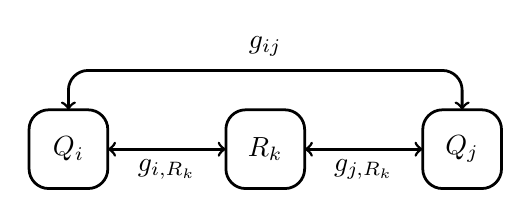
\begin{tikzpicture}[line width=1pt]
            \draw (0,0) pic{res_node={R_k, $R_k$}};
            \draw (-2.5,0) pic{res_node={Qi, $Q_i$}};
            \draw (2.5,0) pic{res_node={Qj, $Q_j$}};
            \draw[<->] (-2,0) -- (-.5,0) node [midway, below] {$g_{i,R_k}$}; 
            \draw[<->] (2,0) -- (.5,0) node [midway, below] {$g_{j,R_k}$};
            \draw[rounded corners=0.25cm, <->] (-2.5,.5) -- (-2.5, 1) -- (2.5,1) -- (2.5,.5);
            \node at (0,1.3) {$g_{ij}$};
        \end{tikzpicture}
        \caption{$g_{ij} \ll g_{i,R_k}, g_{j,R_k}$}
        \label{fig:2Q1R_1}
    \end{subfigure}%
    \begin{subfigure}{.5\textwidth}
        \centering
        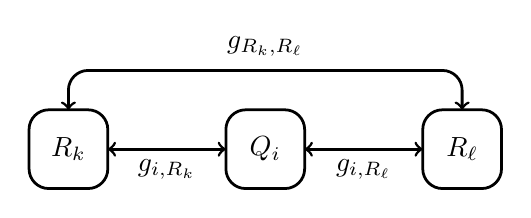
\begin{tikzpicture}[line width=1pt]
            \draw (0,0) pic{res_node={R_k, $Q_i$}};
            \draw (-2.5,0) pic{res_node={Qi, $R_k$}};
            \draw (2.5,0) pic{res_node={Qj, $R_\ell$}};
            \draw[<->] (-2,0) -- (-.5,0) node [midway, below] {$g_{i,R_k}$}; 
            \draw[<->] (2,0) -- (.5,0) node [midway, below] {$g_{i,R_\ell}$};
            \draw[rounded corners=0.25cm, <->] (-2.5,.5) -- (-2.5, 1) -- (2.5,1) -- (2.5,.5);
            \node at (0,1.3) {$g_{R_k,R_\ell}$};
        \end{tikzpicture}
        \caption{$g_{R_k,R_\ell} \ll g_{i,R_k},g_{i,R_\ell}$}
        \label{fig:1Q2R_1}
    \end{subfigure}
    \caption{}
    \label{fig:chain_layout}
\end{figure}

In Fig.\ \ref{fig:2Q1R_1}, we can see an example schematic where two qubits are coupled directly and through a resonant mode. Notably, the direct coupling between the qubits will be much smaller than the coupling between the qubits and the resonator such that $g_{ij} \ll g_{i,R_k}, g_{j,R_k}$. This type of layout is typically found in superconducting circuits with qubit chains or grids coupled by resonators \cite{solgun_sirf,rapid_multiplexed_readout} as well as systems with qubits coupled by tunable couplers \cite{tunable_coupler,high_fidelity_cz_iswap_tc,long_distance_coupler}. For these types of couplings, it is clear that the coefficients $g_{ij}g_{i,R_k}\Delta_{i,R_k}^{-1}$ and $g_{ij}g_{i,R_k}\Sigma_{i,R_k}^{-1}$ in (\ref{eq:comm_H1_Q}) generated by $[\hat{S}_{ik}, \hat{H}^1_{Q,ij}]$  will be small compared to the original term that couples the qubits and resonators, so this contribution can be neglected. If we look at the layout in Fig.\ \ref{fig:1Q2R_1}, we find the condition $g_{R_k,R_\ell} \ll g_{i,R_k},g_{i,R_\ell}$. For this layout, a similar argument can be made for why the new terms in (\ref{eq:comm_H1_R}) generated by $[\hat{S}_{ik}, \hat{H}^1_{R,k\ell}]$ can be neglected as well.

\begin{figure}[h!]
    \centering
    \begin{subfigure}{.4\textwidth}
        \centering
        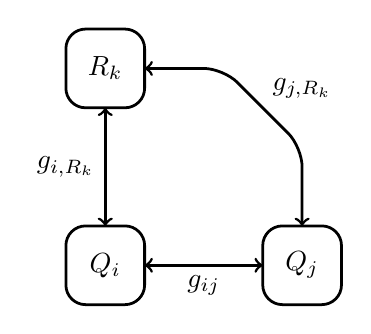
\begin{tikzpicture}[line width=1pt]
            \draw (0,2.5) pic{res_node={R_k, $R_k$}};
            \draw (0,0) pic{res_node={Qi, $Q_i$}};
            \draw (2.5,0) pic{res_node={Qj, $Q_j$}};
            \draw[<->] (0.5,0) -- (2,0) node [midway, below] {$g_{ij}$};
            \draw[<->] (0,.5) -- (0,2) node [midway, left] {$g_{i,R_k}$};
            \draw[rounded corners=0.25cm, <->] (2.5,0.5) -- (2.5,1.5) -- (1.5,2.5) -- (0.5,2.5);
            \node at (2.5, 2.25) {$g_{j,R_k}$};
        \end{tikzpicture}
        \caption{$g_{j,R_k} \ll g_{i,R_k},g_{ij}$}
        \label{fig:2Q1R_2}
    \end{subfigure}%
    \begin{subfigure}{.4\textwidth}
        \centering
        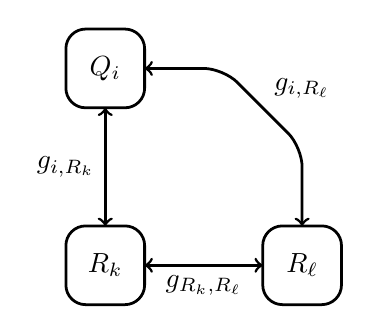
\begin{tikzpicture}[line width=1pt]
            \draw (0,2.5) pic{res_node={R_k, $Q_i$}};
            \draw (0,0) pic{res_node={Qi, $R_k$}};
            \draw (2.5,0) pic{res_node={Qj, $R_\ell$}};
            \draw[<->] (0.5,0) -- (2,0) node [midway, below] {$g_{R_k,R_\ell}$};
            \draw[<->] (0,.5) -- (0,2) node [midway, left] {$g_{i,R_k}$};
            \draw[rounded corners=0.25cm, <->] (2.5,0.5) -- (2.5,1.5) -- (1.5,2.5) -- (0.5,2.5);
            \node at (2.5, 2.25) {$g_{i,R_\ell}$};
        \end{tikzpicture}
        \caption{$g_{i,R_\ell} \ll g_{i,R_k},g_{R_k,R_\ell}$}
        \label{fig:1Q2R_2}
    \end{subfigure}
    \caption{}
    \label{fig:angle_layout}
\end{figure}

While many cases are covered by Fig.\ \ref{fig:2Q1R_1}, this leaves out cases where resonant modes are not used for coupling. For example, Fig.\ \ref{fig:2Q1R_2} represents a layout where one qubit has strong direct coupling to another qubit as well as a resonator that is used for readout. You would have this layout in a capacitively coupled transmon chain where each has its own readout resonator \cite{Barends2016}. It is also clear that the coefficients in (\ref{eq:comm_H1_Q}) will be small under the condition $g_{j,R_k} \ll g_{i,R_k},g_{ij}$ compared to the original qubit-resonator coupling rates. If we consider the layout in Fig.\ \ref{fig:1Q2R_2}, we now have the condition $g_{i,R_\ell} \ll g_{i,R_k},g_{R_k,R_\ell}$ and again we can see that the new terms from (\ref{eq:comm_H1_R}) for this layout can be neglected. This layout will typically be seen in architectures that make use of Purcell filters for readout \cite{rapid_multiplexed_readout,karamlou2023probing}. In the rest of our analysis, we restrict ourselves to chip architectures with the above layouts and constraints on the couplings. While the restrictions are not ideal, it will not pose a problem as most architectures will not violate the above conditions. However, it is good to be wary of these restrictions since the approximations we will now make would break down if they are violated.

Given the restrictions on the circuit layouts that have been discussed, we can further reduce the expansion of the transformed Hamiltonian. We have determined that the new qubit-resonator coupling rates in (\ref{eq:comm_H1_Q}) and (\ref{eq:comm_H1_R}) that come from $[\hat{S},\hat{H}^1]$ can be neglected in the final Hamiltonian. Thus, the transformed Hamiltonian to second order in $g$ with the additional restrictions given our desired circuit layout is:
\begin{equation}
    \hat{U} \hat{H} \hat{U}^\dag \approx \hat{H}^0 + \hat{H}^1 + \frac{1}{2}[\hat{S}, \hat{H}^2]
\end{equation}
We have already found the contributions to the commutator $[\hat{S}, \hat{H}^2]$ in (\ref{eq:qubit_eff_coup_adj}), (\ref{eq:res_eff_coup_adj}) and (\ref{eq:qubit_res_shifts}). This allows us to write the new effective Hamiltonian, and with the approximations we've made, this Hamiltonian will have no coupling between the qubits and resonators. The effective Hamiltonian is:
\begin{align}
\begin{split}\label{eq:eff_ham}
    \hat{H}_{\text{eff}} &\approx \sum_{i=1}^N \left(  \tilde{\omega}_{J_i}\opbd_i\opb + \frac{\beta_{J_i}}{2}\opbd_i\opbd_i\opb_i\opb_i  + \sum_{j > i}^{j=N} \tilde{g}_{ij} (\opbd_i\opb_j + \opb_i\opbd_j - \opbd_i\opbd_j - \opb_i\opb_j) \right) \\
    &\quad + \sum_{k=1}^M \left( \tilde{\omega}_{R_k}\opad_k\opa_k + \frac{\alpha_{R_k}}{2} \opad_k\opad_k\opa_k\opa_k + \sum_{\ell > k}^{\ell=M} \tilde{g}_{R_k,R_\ell} (\opad_k\opa_\ell + \opa_k\opad_\ell - \opad_k\opad_\ell - \opa_k\opa_\ell) \right)
\end{split}
\end{align}
where now the qubit and resonator frequencies as well as the direct coupling rates are shifted. Note that at this point we haven't included any effect of the nonlinear terms and this assumption will hold for $\beta,\alpha \ll \Delta$. In the next section we will see some of the effects that these nonlinear terms have. The shifts to the qubit and resonator frequencies are:
\begin{align}
    \tilde{\omega}_{J_i} &\approx \omega_{J_i} + \sum_{k=1}^M g^2_{i,R_k}\left( \frac{1}{\Delta_{i,R_k}} - \frac{1}{\Sigma_{i,R_k}} \right) \label{eq:eff_qubit_freq} \\
    \tilde{\omega}_{R_k} &\approx \omega_{R_k} - \sum_{i=1}^N g^2_{i,R_k}\left( \frac{1}{\Delta_{i,R_k}} + \frac{1}{\Sigma_{i,R_k}} \right) \label{eq:eff_res_freq}
\end{align}
Note that in the above we have left out the high frequency rotating terms that arise in (\ref{eq:qubit_res_shifts}). The new effective direct coupling terms are defined as follows:
\begin{align}
    \tilde{g}_{ij} &\approx g_{ij} + \frac{1}{2} \sum_{k=1}^M  g_{i,R_k}g_{j,R_k} \left( \frac{1}{\Delta_{i,R_k}} + \frac{1}{\Delta_{j,R_k}}  - \frac{1}{\Sigma_{i,R_k}} - \frac{1}{\Sigma_{j,R_k}}\right) \label{eq:eff_qubit_coupling}\\
    \tilde{g}_{R_k,R_\ell} &\approx g_{R_k,R_\ell} - \frac{1}{2}\sum_{i=1}^N g_{i,R_k}g_{i,R_\ell} \left( \frac{1}{\Delta_{i,R_k}} + \frac{1}{\Delta_{i,R_\ell}} + \frac{1}{\Sigma_{i,R_k}} + \frac{1}{\Sigma_{i,R_\ell}} \right)
\end{align}
The results for the frequency shifts and effective coupling closely resemble the results of \cite{tunable_coupler,tunable_coupler_ext}, except now there is a sum component that adds the contributions of all the couplers or qubits that are present. The resulting expression is no real surprise, but here we have shown that a multi-qubit multi-coupler system can be treated in the above way to estimate effective couplings between the qubits.

This final result shows us that starting from a rational impedance function (\ref{eq:impedance}) or a CL cascade network representation of our multi-qubit circuit, we can estimate the effective coupling rates between qubits. If we are able to obtain the rational impedance function from an electromagnetic model of your device, then the remaining characterization process is straightforward given the above formulas. Another useful feature of the above process is that designating some of the qubits as tunable couplers does not change the process or the resulting formulas for the estimated effective coupling.

\subsection{Effects of the Nonlinear Terms}
We now find the effects of the nonlinear terms that were neglected in the last section. We are primarily concerned with finding approximations to the shifts to the qubit and coupler anharmonicities, as well as the state dependent dispersive shifts for the qubits and couplers. To do this, we find how the operators $\opb_i$ and $\opa_k$ are transformed by the operator $\hat{U}$ in (\ref{eq:sw_transform}). To do this, we expand the transformations of these operators perturbatively. Then we can obtain the relevant terms that were previously neglected. We can again use the \ref{eq:BCH} and expand to the second order commutator term which gives:
\begin{equation}
    \hat{U}\opb_i \hat{U}^\dag \approx \opb_i + [\hat{S},\opb_i] + \frac{1}{2}[\hat{S}, [\hat{S},\opb_i]]
\end{equation}
A similar expansion is used for $\opa_k$. The operator $\opb_i$ transformed with this expansion is:
\begin{equation}
    \hat{U}\opb_i \hat{U}^\dag \approx \opb_i - \sum_{k=1}^M g_{i,R_k} \left( \frac{1}{\Delta_{i,R_k}} \opa_k - \frac{1}{\Sigma_{i,R_k}} \opad_k \right) - \frac{1}{2}\sum_{j=1}^N \sum_{k=1}^M \frac{g_{i,R_k}g_{j,R_k}}{\Delta_{i,R_k}\Delta_{j,R_k}} \opb_j
\end{equation}
where we have also neglected terms of order $g^2/(\Delta\Sigma)$ and $g^2/\Sigma^2$ or higher. A similar expansion can be found for the transformed $\opa_k$:
\begin{equation}
    \hat{U}\opa_k \hat{U}^\dag \approx \opa_k + \sum_{i=1}^N g_{i,R_k} \left( \frac{1}{\Delta_{i,R_k}}\opb_i + \frac{1}{\Sigma_{i,R_k}}\opbd_i \right) - \frac{1}{2}\sum_{i=1}^N\sum_{\ell=1}^M \frac{g_{i,R_k}g_{i,R_\ell}}{\Delta_{i,R_k}\Delta_{i,R_\ell}} \opa_{\ell}
\end{equation}
We can now take the above expressions and substitute them into the original nonlinear terms in $\hat{H}^{NL}$ (\ref{eq:H_nonlinear}). To start, we show an example of finding the dispersive shifts to resonator $k$ that come from qubit $i$ and the term $(\beta_i/2)\opbd_i\opbd_i\opb_i\opb_i$. We can substitute the relevant terms from the above transformed $\opb_i$ into this nonlinear term to get:
\begin{equation}
    \frac{\beta_{J_i}}{2}\opbd_i\opbd_i\opb_i\opb_i \quad\longrightarrow\quad \frac{\beta_{J_i}}{2}\left( \opbd_i - \frac{g_{i,R_k}}{\Delta_{i,R_k}}\opad_k + \frac{g_{i,R_k}}{\Sigma_{i,R_k}}\opa_k\right)^2\left(  \opb_i - \frac{g_{i,R_k}}{\Delta_{i,R_k}}\opa_k + \frac{g_{i,R_k}}{\Sigma_{i,R_k}}\opad_k \right)^2
\end{equation} 
In the following, we will not be concerned with any non-resonant terms that come out of the expansions. The terms we will be concerned with provide contributions to the dispersive shift as well as a new additional shift to the qubit frequency. Expanding the nonlinear term for the resonator (if $\alpha_{R_k} \neq 0$), will provide another contribution to both the dispersive shift and another shift to that resonators frequency. The new dispersive shift terms that will be added to the effective Hamiltonian (\ref{eq:eff_ham}) are:
\begin{equation}\label{eq:dispersive_shifts}
    \hat{H}_{\text{eff}}^{DS} = \sum_{i=1}^N \sum_{k=1}^M 2g_{i,R_k}^2 (\beta_{J_i} + \alpha_{R_k}) \left( \frac{1}{\Delta_{i,R_k}^2} + \frac{1}{\Sigma_{i,R_k}^2} \right) \opbd_i\opb_i \opad_k\opa_k
\end{equation}
The new qubit and resonator shifts (\ref{eq:eff_qubit_freq}) and (\ref{eq:eff_res_freq}) are now shifted further (although it is a small amount compared to the first shift):
\begin{align}
    \tilde{\omega}_{J_i} &\approx \omega_{J_i} + \sum_{k=1}^M g^2_{i,R_k}\left( \frac{1}{\Delta_{i,R_k}} - \frac{1}{\Sigma_{i,R_k}} \right) + 2\beta_{J_i} \frac{g_{i,R_k}^2}{\Sigma_{i,R_k}^2} \\
    \tilde{\omega}_{R_k} &\approx \omega_{R_k} - \sum_{i=1}^N g^2_{i,R_k}\left( \frac{1}{\Delta_{i,R_k}} + \frac{1}{\Sigma_{i,R_k}} \right) + 2\alpha_{R_k} \frac{g_{i,R_k}^2}{\Sigma_{i,R_k}^2}
\end{align}
%There are also dispersive shifts between the qubits, but they are of order $\beta g^4/\Delta^4$ so we ignore them here. 
We can also now estimate the shifts to the nonlinear terms that are originally present in the Hamiltonian. To do this, consider again substituting the relevant terms from the transformed $\opb_i$ into the original nonlinear term
\begin{equation}
    \frac{\beta_{J_i}}{2}\opbd_i\opbd_i\opb_i\opb_i \quad\longrightarrow\quad \frac{\beta_{J_i}}{2}\left( \opbd_i - \frac{1}{2}\sum_{j=1}^N \sum_{k=1}^M \frac{g_{i,R_k}g_{j,R_k}}{\Delta_{i,R_k}\Delta_{j,R_k}} \opbd_j\right)^2\left(  \opb_i - \frac{1}{2}\sum_{j=1}^N \sum_{k=1}^M \frac{g_{i,R_k}g_{j,R_k}}{\Delta_{i,R_k}\Delta_{j,R_k}} \opb_j \right)^2
\end{equation} 
Doing the same for any nonlinear resonators, we get the following effective anharmonicities for the qubits and nonlinear resonators that can be substituted into the effective Hamiltonian (\ref{eq:eff_ham}):
\begin{align}
    \tilde{\beta}_{J_i} &\approx \beta_{J_i}\left( 1 - 2\sum_{k=1}^{M} \frac{g_{i,R_k}^2}{\Delta_{i,R_k}^2} \right) \\
    \tilde{\alpha}_{R_k} &\approx \alpha_{R_k}\left( 1 - 2\sum_{i=1}^N \frac{g_{i,R_k}^2}{\Delta_{i,R_k}^2} \right)
\end{align}
Using both of the above approximations for the transformed nonlinear terms, we also find another contribution to the effective Hamiltonian in the form of cross-Kerr terms for the qubits:
\begin{equation}
    \hat{H}_{\text{eff}}^{CK} = \frac{1}{2}\sum_{i=1}^{N}\sum_{j > i}^{j=N}\sum_{k=1}^M \left( \frac{g_{i,R_k}g_{j,R_k}}{\Delta_{i,R_k}\Delta_{j,R_k}} \right)^2 (\beta_{J_i} + \beta_{J_j} + 4\alpha_{R_k}) \opbd_i\opb_i\opbd_j\opb_j
\end{equation}
A similar term exists for the nonlinear resonators with the roles of the qubits and resonators swapped. Once again, these results and approximations do not differ much from the results of \cite{tunable_coupler_ext}, except that we have now shown that these formulas apply to systems with an arbitrary number of qubits and resonators. It is also possible to apply further transformations to eliminate any non-resonant terms that we have neglected as was done in \cite{tunable_coupler_ext}. Here, we will not go further as these transformations would eliminate the dispersive shift terms and what we have shown should be enough to estimate the relevant parameters when designing a chip.
